% Original Phase 2 research proposal, formatted in IEEEtran conference style.
% Official template: https://conferences.ieeeauthorcenter.ieee.org/write-your-paper/authoring-tools-and-templates/
% IEEEtran class by Michael Shell; standard class distributed through TeX Live/MiKTeX.
% Standalone source: no external images, .bib files, or project inputs.
\documentclass[conference]{IEEEtran}
\usepackage[T1]{fontenc}
\usepackage{cite}
\usepackage{amsmath,amssymb}
\usepackage{array,booktabs}
\usepackage{tikz}
\usetikzlibrary{arrows.meta,positioning,calc,fit}
\usepackage[hidelinks]{hyperref}
\urlstyle{same}
\hypersetup{pdftitle={Machine Learning-Based Detection of Previously Unseen Low-Rate DDoS Attacks},pdfauthor={M Abdullah Nadeem and Ayaan Faisal},pdfsubject={Computer Networks Phase 2 research proposal}}
\hyphenation{auto-encoder auto-encoders data-sets Slow-loris Slow-http-test}
\begin{document}
\title{Machine Learning-Based Detection of Previously Unseen Low-Rate DDoS Attacks}
\author{\IEEEauthorblockN{M Abdullah Nadeem}
\IEEEauthorblockA{Computer Networks}
\and
\IEEEauthorblockN{Ayaan Faisal}
\IEEEauthorblockA{Computer Networks}}
\maketitle
% Page numbers aid review of this course proposal; no conference metadata is claimed.
\pagestyle{plain}
\thispagestyle{plain}
\begin{abstract}
Previously unseen slow denial-of-service traffic can resemble legitimate low-volume activity, while benign bursts can trigger anomaly-based alarms. This Phase 2 proposal extends the completed literature review with eight original research articles published in 2025--2026. The review shows that hybrid detection and strict zero-day holdouts already exist; the remaining question concerns their joint reliability under excluded slow-attack families, benign stress, and environment transfer at a threshold fixed before testing. We propose a compact supervised detector combined with a benign-trained autoencoder, using causal destination-service windows and separate score-reference and threshold-calibration sets. The planned evaluation reports per-family recall, ordinary and stressed-traffic false positives, episode detection delay, matched baselines, statistical uncertainty, and component ablations. A twelve-step methodology and architecture diagram define the experimental protocol. This document reports a research plan and author-reported literature results; no project experiments have yet been performed.
\end{abstract}
\begin{IEEEkeywords}
low-rate DDoS, slow DoS, unseen attacks, intrusion detection, autoencoder, false positives, research methodology
\end{IEEEkeywords}

\section{Introduction}
\label{sec:intro}
Slow denial-of-service activity may consume connection or application resources without producing a conspicuous traffic spike. Detection must therefore be assessed against legitimate traffic that is both ordinary and unusually busy. The Phase 1 foundation considers generalized DDoS detection, unsupervised slow-DoS detection and early low-rate attack recognition \cite{ref1,ref2,ref3}.

We propose a reproducible evaluation of whether a compact machine-learning intrusion detection system can recognize previously unseen slow denial-of-service behaviour while maintaining a low false-positive rate on ordinary and stressed legitimate traffic. The candidate detector combines supervised learning on known attacks with an autoencoder trained on benign observations. Its contribution is a controlled evaluation of attack novelty, low-rate behaviour, benign stress and detection delay together; superior performance is a hypothesis to test.

Eight additional research articles from 2025-2026 extend the three Phase 1 papers. The extended review refines the original gap because recent studies already provide hybrid detectors and strict zero-day holdouts. The proposed work concentrates on the remaining operating tradeoff and the quality of the evidence used to measure it.

The project remains limited to detection and evaluation. Its output is a timestamped alert with supporting scores. Automatic blocking, rate limiting, traffic redirection and mitigation-effectiveness experiments are outside the implementation scope.

The proposal contributes four assignment deliverables: an extended critical literature review (Section II), an evidence-based refined gap (Section III), a twelve-step proposed methodology (Section IV), and a research architecture diagram (Section V). Section VI addresses feasibility and validity. The paper is prepared for the Computer Networks Phase 2 submission, revised 17 October 2026.

\section{Extended Literature Review}
\label{sec:review}
\subsection{Selection and Venue Eligibility}
The search covered publisher article pages and accessible author manuscripts using combinations of low-rate DDoS, slow DoS, zero-day intrusion detection, autoencoder, temporal detection, false positives and lightweight classification. Inclusion required an original 2025-2026 research article, a Q1-Q2 venue under the stated ranking system, and identifiable data, method and evaluation. Surveys, editorials, duplicate records and papers without usable experimental information were excluded. This is a focused critical review rather than a claimed exhaustive systematic review.

The eight additions A1-A8 below are distinct from the Phase 1 studies by Bocu and Iavich \cite{ref1}, Rullo et al. \cite{ref2} and Nakip \cite{ref3}. A4 and A7 contribute directly relevant DDoS classifier baselines and evaluation lessons; they are not treated as evidence that unseen low-rate attacks have been solved. Dataset documentation is supporting material and is not counted toward the eight articles.

Quartiles below use SCImago SJR, not JCR. The audited 2024 edition provides a common documented basis: IEEE Access Q1, Scientific Reports Q1, Results in Engineering Q1 and Computers, Materials \& Continua Q2 \cite{ref15,ref16,ref17,ref18}. The latter is JCR Q3 in 2024, so its eligibility here specifically depends on SJR Q2. The assignment does not name a ranking system. The 2025 institutional records also list Results in Engineering Q1 and CMC Q2 \cite{ref17,ref18}.

A8 was first published online on 29 December 2025; the publisher cites volume 16, article 2305 as 2026. Both dates fall within the required interval \cite{ref11}. Publication years are verified from article records, independently of venue-ranking years.

\subsection{Critical Review of Eight Additional Studies}
\subsubsection{A1 Minhas and colleagues 2025}
F-OSFA proposes a CNN/decision-tree classifier, a benign-trained contractive autoencoder and a resource-use analyser. Its abstract reports zero-day accuracies of 96.77\% on CIC-DDoS2019 and 95.98\% on CIC-IDS2017. However, its future-work section still calls for a resource-labelled dataset to implement the resource analyser, so those headline results do not establish validation of every proposed component. The abstract's few-shot terminology also differs from the methodology's zero-shot module. Hybrid detection is therefore established, while unseen slow-family recall at a fixed benign-stress false-positive budget remains a distinct evaluation question \cite{ref4}.

\subsubsection{A2 Ullah and colleagues 2026}
The dual-head framework combines supervised classification with anomaly detection, uses dataset-adaptive minority augmentation including WGAN-GP, and supplies SHAP explanations. CIC-IoT2023, BoT-IoT and ToN-IoT experiments include a true zero-day holdout, component ablations and five-seed validation. The paper reports accuracy and F1 above 99.5\% across its evaluated datasets and approximately 0.5 MB model size. Therefore, a claim that recent IDS research lacks strict holdouts is no longer defensible. Its broad intrusion results do not establish the specific unseen slow-attack versus benign-stress tradeoff investigated here. Reported per-sample inference cost also cannot replace attack-onset-to-alert delay \cite{ref5}.

\subsubsection{A3 Han and colleagues 2025}
CA-CAE uses consecutive asymmetric convolutional autoencoders with joint reconstruction and a score weighted by recency and relative traffic volume. Cisco NetFlow measurements contain 190,817 normal and 78 anomalous instances; the reported F1 rises from 0.515 for the baseline CAE to 0.934. Differencing and overlapping windows make this relevant to temporal anomaly detection. However, volume weighting requires testing when an attack deliberately has low volume, and only 78 anomalies constrain uncertainty estimates. The counts imply about 0.041\% anomalies, rather than the 0.0004\% printed in the article. This arithmetic discrepancy should not be propagated into our experimental design \cite{ref6}.

\subsubsection{A4 Nawaz and colleagues 2025}
This study compares Random Forest, Logistic Regression and Naive Bayes after cleaning, encoding, scaling and ExtraTrees selection of 18 features from NSL-KDD. It reports Random Forest accuracy of 99.88\% and F1 of 99.87\%, using an 80:20 split and tenfold validation. It provides a useful justification for including inexpensive classical baselines rather than assuming deep learning is necessary. The authors acknowledge that NSL-KDD is not IoT-specific and may not represent current traffic. Neither conventional cross-validation nor this dataset establishes unseen low-rate DDoS detection. We retain the baseline lesson while selecting slow-attack traces and temporally separated sessions for our own evaluation \cite{ref7}.

\subsubsection{A5 Anandhi and Srikanth 2026}
FSL-IDS targets low-rate stealth attacks through sparse local encoding, fog-level temporal correlation and cloud aggregation, with training-only synthetic stealth augmentation and quantization. The authors report IoTID20-based experiments, cloud ROC-AUC 0.992 and F1 0.965, plus substantial recall loss when augmentation is removed. This makes temporal context and component ablation relevant to our design. However, the reported stealth labels and augmented data require provenance auditing; they should not automatically be treated as native benchmark categories. Exposure to stealth samples during training also differs from excluding an entire slow-attack family. Our evaluation therefore separates attack novelty from rarity and records the origin of every label \cite{ref8}.

\subsubsection{A6 Raza and colleagues 2026}
This work combines liquid time-constant layers and attention, independently training and evaluating on SNT-SDN2025, CICIoT2023 and IoT23. Cleaning and standardization precede ten-flow sequences; a chronological 70:30 split is made before window generation. The maximum reported accuracy is 99.96\%, with 0.07\% FPR on CICIoT2023. The temporal separation is a useful leakage-control pattern. However, independently fitting a model on each dataset is not frozen-model cross-dataset transfer, and future traffic is not necessarily a new attack family. We adopt the split-before-window principle and evaluate both novelty and transfer explicitly rather than treating temporal modelling alone as evidence of either \cite{ref9}.

\subsubsection{A7 Ebrahem and colleagues 2026}
The paper studies compact feature subsets with Random Forest, KNN, Complement Naive Bayes and Logistic Regression on CIC-DDoS2019, using LDAP, MSSQL, UDP and benign traffic. It removes identifying metadata, cleans invalid values, encodes labels and compares NearMiss-balanced and imbalanced experiments. Table 23 reports RF accuracy 99.32\% and F1 99.40\%. This supports compact baselines and reporting computational cost. Its documented balancing-before-splitting workflow warrants a leakage audit, and the selected flooding classes do not certify slow-attack performance. In our pipeline, every learned transformation and any resampling occur strictly within training, while test prevalence is preserved \cite{ref10}.

\subsubsection{A8 Kalafy and colleagues 2026}
GCTNetwork integrates gated temporal graph layers, edge-aware LSTM and graph attention on an SDN testbed-derived flow dataset. It applies log transforms, min-max scaling and graph construction, reporting 94.08\% accuracy and 93.27\% F1 against ST-GCN, GRAN and LR-STGCN. Graph context is relevant to coordinated activity that individual flows may hide. However, the presented classes are benign and ICMP/TCP/UDP floods, rather than a dedicated unseen slow-family evaluation. The training configuration states ten epochs while the learning-curve discussion describes 100, creating a reproducibility ambiguity. Our simpler aggregation retains temporal context with explicit settings and matched comparisons \cite{ref11}.

\begin{table*}[!t]
\caption{Cross-paper comparison of additional studies A1--A4. All results are author-reported on different tasks and datasets; they do not establish a performance ranking.}
\label{tab:review1}
\centering\footnotesize\setlength{\tabcolsep}{2.2pt}\renewcommand{\arraystretch}{1.12}
\begin{tabular}{@{}>{\raggedright\arraybackslash}p{\dimexpr 0.03371\textwidth-1.187pt\relax}>{\raggedright\arraybackslash}p{\dimexpr 0.18539\textwidth-6.526pt\relax}>{\raggedright\arraybackslash}p{\dimexpr 0.05393\textwidth-1.898pt\relax}>{\raggedright\arraybackslash}p{\dimexpr 0.11798\textwidth-4.153pt\relax}>{\raggedright\arraybackslash}p{\dimexpr 0.13708\textwidth-4.825pt\relax}>{\raggedright\arraybackslash}p{\dimexpr 0.12135\textwidth-4.271pt\relax}>{\raggedright\arraybackslash}p{\dimexpr 0.10899\textwidth-3.836pt\relax}>{\raggedright\arraybackslash}p{\dimexpr 0.11011\textwidth-3.876pt\relax}>{\raggedright\arraybackslash}p{\dimexpr 0.13146\textwidth-4.627pt\relax}@{}}\toprule
\textbf{\#} & \textbf{Title} & \textbf{Year} & \textbf{Dataset used} & \textbf{Preprocessing techniques} & \textbf{Models or techniques} & \textbf{Evaluation metrics} & \textbf{Results} & \textbf{Limitations or research gap}\\\midrule
A1 & F-OSFA: A Fog Level Generalizable Solution for Zero-Day DDOS Attacks Detection \cite{ref4} & 2025 & CIC-DDoS2019; CIC-IDS2017 & Metadata/constant removal; invalid-value cleaning; min-max scaling & CNN + decision tree; contractive AE; proposed resource analyser & Accuracy; precision; recall; F1; FPR & Zero-day accuracy 96.77\% / 95.98\% & Resource-prong evidence limited; slow/stress tradeoff not established\\
\addlinespace[4pt]
A2 & Hybrid dual-head IDS: A lightweight and explainable deep learning DDOS/DOS framework for zero-day and imbalanced attack detection in IoT networks \cite{ref5} & 2026 & CIC-IoT2023; BoT-IoT; ToN-IoT & Training-only adaptive augmentation; fitted preprocessing & Dual heads; hybrid loss; SHAP & Accuracy; F1; ROC-AUC; ZDS; inference time & >99.5\% accuracy/F1; about 0.5 MB & Strict holdout exists; slow-attack stress tradeoff remains distinct\\
\addlinespace[4pt]
A3 & Adapting Convolutional Autoencoder for DDoS Attack Detection via Joint Reconstruction Learning and Refined Anomaly Scoring \cite{ref6} & 2025 & Cisco NetFlow; 190,817 normal; 78 anomalous & First differences; standardization; overlapping windows & Two asymmetric CAEs; temporal and volume scoring & Precision; recall; F1; statistical comparisons & F1 0.934 versus baseline 0.515 & Rare anomalies; volume weighting may underweight slow attacks\\
\addlinespace[4pt]
A4 & Lightweight machine learning framework for efficient DDoS attack detection in IoT networks \cite{ref7} & 2025 & NSL-KDD & Cleaning; encoding; scaling; ExtraTrees top 18 & Random Forest; Logistic Regression; Naive Bayes & Accuracy; precision; recall; F1; fold variation & RF accuracy 99.88\%; F1 99.87\% & Legacy non-IoT benchmark; unseen slow attacks not established\\
\bottomrule\end{tabular}
\end{table*}

\begin{table*}[!t]
\caption{Cross-paper comparison of additional studies A5--A8, using the same nine assignment fields.}
\label{tab:review2}
\centering\footnotesize\setlength{\tabcolsep}{2.2pt}\renewcommand{\arraystretch}{1.12}
\begin{tabular}{@{}>{\raggedright\arraybackslash}p{\dimexpr 0.03371\textwidth-1.187pt\relax}>{\raggedright\arraybackslash}p{\dimexpr 0.18539\textwidth-6.526pt\relax}>{\raggedright\arraybackslash}p{\dimexpr 0.05393\textwidth-1.898pt\relax}>{\raggedright\arraybackslash}p{\dimexpr 0.11798\textwidth-4.153pt\relax}>{\raggedright\arraybackslash}p{\dimexpr 0.13708\textwidth-4.825pt\relax}>{\raggedright\arraybackslash}p{\dimexpr 0.12135\textwidth-4.271pt\relax}>{\raggedright\arraybackslash}p{\dimexpr 0.10899\textwidth-3.836pt\relax}>{\raggedright\arraybackslash}p{\dimexpr 0.11011\textwidth-3.876pt\relax}>{\raggedright\arraybackslash}p{\dimexpr 0.13146\textwidth-4.627pt\relax}@{}}\toprule
\textbf{\#} & \textbf{Title} & \textbf{Year} & \textbf{Dataset used} & \textbf{Preprocessing techniques} & \textbf{Models or techniques} & \textbf{Evaluation metrics} & \textbf{Results} & \textbf{Limitations or research gap}\\\midrule
A5 & Federated sparse-learning framework for detecting low-rate stealth attacks in resource-constrained IoT devices \cite{ref8} & 2026 & IoTID20-based traffic; reported LRSA subset & Filtering; sessionization; min-max; training augmentation & Sparse AE; fog temporal ensemble; federated aggregation & ROC-AUC; F1; LRSA recall; latency; energy & Cloud AUC 0.992; F1 0.965 & Audit stealth-label provenance; rarity differs from novelty\\
\addlinespace[4pt]
A6 & Liquid neural networks for adaptive DDoS detection in IoT and SDN environments \cite{ref9} & 2026 & SNT-SDN2025; CICIoT2023; IoT23 & Clean; standardize; temporal split before 10-flow windows & Liquid time-constant network + attention & Accuracy; precision; recall; FPR; FNR; robustness & Maximum accuracy 99.96\%; FPR 0.07\% & Separate dataset fitting does not prove frozen transfer\\
\addlinespace[4pt]
A7 & A lightweight machine learning approach for DDoS detection and classification \cite{ref10} & 2026 & CIC-DDoS2019 subset: LDAP, MSSQL, UDP, benign & Metadata removal; invalid-value cleaning; NearMiss & RF; KNN; Complement NB; Logistic Regression & Accuracy; precision; recall; F1; FPR; time; memory & Table 23 RF accuracy 99.32\%; F1 99.40\% & Audit resampling order; flooding subset is not slow evidence\\
\addlinespace[4pt]
A8 & Dynamic graph neural network-based framework to increase detection accuracy in SDN under DDOS \cite{ref11} & 2026 & SDN flow dataset from Mininet, POX and OVS & log1p; min-max; encoding; node/edge aggregation & Gated temporal graph layers; edge LSTM; GAT & Accuracy; precision; recall; F1; DR; FAI & Accuracy 94.08\%; F1 93.27\% & Flood classes; no dedicated unseen slow-family result\\
\bottomrule\end{tabular}
\end{table*}

\subsection{Cross-Paper Synthesis and Design Implications}
The review identifies four established approaches: classical supervised flow classification; benign-trained reconstruction or one-class detection; hybrid known-attack and anomaly branches; and temporal or graph modelling of coordinated behaviour. Feature cleaning, reduced representations and thresholded scores recur, but they address different experimental questions. A random or stratified split measures recognition within a sampled distribution; a time split measures later traffic; a family holdout measures attack novelty; and frozen transfer measures change of environment. These should be reported separately \cite{ref4,ref5,ref6,ref7,ref8,ref9,ref10,ref11}.

\noindent\textit{Hybrid and zero-day detection already exist \cite{ref4,ref5}.} Use a modest hybrid as a testable candidate; locate the contribution in the evaluation problem.

\noindent\textit{Temporal representations can expose subtle activity \cite{ref6,ref8,ref9,ref11}.} Use fixed-time destination aggregates and strictly causal rolling features.

\noindent\textit{Compact classifiers can be competitive \cite{ref7,ref10}.} Include Logistic Regression and Random Forest baselines.

\noindent\textit{Reconstruction and augmentation choices influence performance \cite{ref5,ref6,ref8}.} Measure the effect of each branch and temporal component; avoid synthetic attack augmentation in the core study.

\noindent\textit{Published metrics use different datasets and units \cite{ref4,ref5,ref6,ref7,ref8,ref9,ref10,ref11}.} Do not rank papers by their headline accuracy; compare our implementations on identical splits.

The earlier broad gap about an absence of strict unseen-attack protocols must be narrowed: A2 explicitly includes such a protocol \cite{ref5}. Our central question becomes whether unseen slow attacks can be detected at a threshold fixed before testing while legitimate bursts and congestion remain below an acceptable false-alarm level. The study also asks what temporal observation costs are required to obtain that performance.

Tables I and II retain the nine comparison fields required by the assignment. AE denotes autoencoder; CAE, convolutional autoencoder; FAI, false alarm index; ZDS, zero-day separation; LRSA, low-rate stealth attack; and DR, detection rate. Limitations are our critical interpretations unless attributed to the original authors.

Interpretation: attack-family novelty, low traffic volume and temporal distribution change are different properties. High accuracy in one does not establish performance in the others. We therefore use explicit holdout and stress-test definitions rather than transferring headline results to the proposed task.

\section{Refined Research Gap}
\label{sec:gap}
Existing work already demonstrates high benchmark accuracy, benign-trained anomaly detection, hybrids, temporal representations and strict holdouts. The narrower opportunity is to measure their joint reliability when an excluded slow-attack family and unusual legitimate traffic are both encountered after thresholds are frozen. The table triangulates four potential gaps using three especially relevant additions; it does not claim that every prior paper omits every experiment.

\begin{table*}[!t]
\caption{Four potential research gaps triangulated against three relevant additional studies. Existing capabilities are acknowledged explicitly.}
\label{tab:gaps}
\centering\footnotesize\setlength{\tabcolsep}{2.2pt}\renewcommand{\arraystretch}{1.12}
\begin{tabular}{@{}>{\raggedright\arraybackslash}p{\dimexpr 0.18657\textwidth-3.284pt\relax}>{\raggedright\arraybackslash}p{\dimexpr 0.15672\textwidth-2.758pt\relax}>{\raggedright\arraybackslash}p{\dimexpr 0.15672\textwidth-2.758pt\relax}>{\raggedright\arraybackslash}p{\dimexpr 0.15672\textwidth-2.758pt\relax}>{\raggedright\arraybackslash}p{\dimexpr 0.34328\textwidth-6.042pt\relax}@{}}\toprule
\textbf{Research gap} & \textbf{A1 F OSFA \cite{ref4}} & \textbf{A2 Dual head \cite{ref5}} & \textbf{A5 FSL IDS \cite{ref8}} & \textbf{Research opportunity}\\\midrule
G1 Joint novelty and benign stress & Zero-day batches exist & True holdout exists & Stealth learning uses examples & Test an excluded slow family and reserved benign-stress sessions at the same frozen threshold\\
\addlinespace[4pt]
G2 Temporal evidence versus delay & Multiple proposed detection prongs & Fast sample inference reported & Temporal aggregation is central & Separate observation wait, feature cost and inference from onset-to-alert delay\\
\addlinespace[4pt]
G3 Provenance and transfer & Two public CIC datasets & Three IoT benchmarks & Stealth-label audit needed & Publish a label map and split manifest; perform frozen external testing on compatible features\\
\addlinespace[4pt]
G4 Complexity versus value & Three proposed prongs; resource validation limited & Dual heads and adaptive augmentation & IoT-fog-cloud hierarchy & Compare a compact hybrid with simple baselines and isolate component gains\\
\bottomrule\end{tabular}
\end{table*}

\subsection{Central Gap and Research Justification}
Within the reviewed studies, evidence remains insufficient to establish whether a compact, reproducible detector can maintain useful recall on a completely excluded slow-attack family while respecting a threshold calibrated to at most 1\% false positives on development benign traffic, and how that operating point changes under reserved benign stress and network transfer. This is an evaluation and generalization gap, not a claim of inventing hybrid detection or the first zero-day protocol.

An IDS that reacts to every legitimate burst can generate an impractical number of alerts; a detector that waits for a completed long connection may recognize a slow attack too late. We will hold out complete families, fit all preprocessing only on training, calibrate on separate benign sessions, freeze the full pipeline, and report per-family recall, stress FPR and onset-to-alert delay. Negative findings will identify the boundary of the method rather than be hidden by average accuracy.

\subsection{Research Questions and Objectives}
Can a compact supervised-plus-anomaly IDS detect previously unseen slow DoS-DDoS behaviour at a low false-positive operating point, including on stressed legitimate traffic, with acceptable observation and computation delay?

\noindent\textit{RQ1 Unseen attack detection.} O1 Exclude the Slowloris and Slowhttptest group completely from development and measure final recall. Per-family and macro recall; episode recall; confusion counts.

\noindent\textit{RQ2 False positives.} O2 Calibrate the final decision to development FPR $\leq$1\% in both ordinary and stressed benign strata; measure held-out FPR separately. FPR, FP count and benign denominator for each workload.

\noindent\textit{RQ3 Value of components.} O3 Compare the hybrid with each branch and classical baselines using matched inputs and splits. Paired recall/FPR differences and cluster-level intervals.

\noindent\textit{RQ4 Delay and transfer.} O4 Measure lab onset-to-alert delay and apply the frozen pipeline to a completely reserved compatible external dataset. Detected and missed episodes; delay distribution; external recall and FPR.

\subsection{Definitions, Hypotheses, and Claim Boundaries}
Previously unseen means the test family is absent from training, model selection, threshold calibration and attack augmentation. It does not mean an unknown software vulnerability. A time split alone is insufficient. Low-rate status must be supported by the attack mechanism and measured traffic rates; a random low-percentile sample from a flood dataset will not be relabelled as a genuine low-rate attack.

H1: the hybrid improves excluded-family recall over the supervised branch at its matched development FPR. H2: causal temporal context improves unseen slow-attack episode recall over instantaneous features. H3: persistence reduces benign-stress alerts, with a measurable delay cost. These are testable hypotheses, not assumed outcomes.

CIC-IDS2017 Slowloris and Slowhttptest support slow DoS evidence \cite{ref12}. Distributed low-rate DDoS claims additionally require multiple independently logged source clients in the isolated lab. Offline CSV classification cannot establish live detection latency. Likewise, an unusual low-rate malicious trace without measured service degradation supports detection of attack attempts, not successful denial of service. Broader Internet or production IoT effectiveness will remain outside the demonstrated scope.

\section{Proposed Research Methodology}
\label{sec:method}
The following twelve steps operationalize the research questions. All numerical settings are proposed design choices, to be finalized using development data before the final evaluation. The workflow in Fig. 1 separates learning and calibration from final tests.

\subsection{Step 1 Define the research input}
The primary input is timestamped packet metadata grouped by destination service into non-overlapping one-second windows. Each record retains dataset, capture, session, attack family, time, traffic-condition and label provenance for splitting and evaluation; identifiers are not predictive features. The online feature builder uses only packets already observed. Rolling context uses the preceding ten seconds, with shorter and longer histories considered on development data only.

The binary target is benign versus attack-associated activity, with original attack families retained for reporting. A positive window must contain attack packets identified by audited flow/packet labels or lab event logs; time inside a scheduled attack interval alone is insufficient. Reconcile time zones, flow direction, five-tuples and NAT mappings before joining labels. Retain ambiguous mixed windows in a separate sensitivity analysis with their counts. Episode timing follows logged attack start/end; service availability and response-time logs evaluate lab impact but are not model inputs.

\subsection{Step 2 Data collection}
\noindent\textit{CIC-IDS2017 \cite{ref12}.} Primary public data; benign, Hulk, GoldenEye, DDoS, Slowloris and Slowhttptest; exclude unrelated intrusion types. Provides PCAP, flow labels and attack schedule, including named slow DoS.

\noindent\textit{CSE-CIC-IDS2018 \cite{ref13}.} Entire source reserved for frozen external testing on compatible benign and slow DoS records; no target-benign calibration in the primary experiment. Different capture environment with slow DoS scenarios.

\noindent\textit{CIC-DDoS2019 \cite{ref14}.} Secondary known/flood-family benchmark in a separate experiment. Multiple DDoS families; not treated as sufficient slow-attack evidence.

\noindent\textit{Isolated local lab.} Mandatory benign-stress and multi-source slow-traffic sessions. Controls workload, distributed sources, intensity and service impact.

Before modelling, build a manifest containing source URLs, downloaded file hashes, extraction version, label map, family aliases, usable sample counts and session IDs. Reconcile labels against schedules and capture metadata; retain excluded/ambiguous counts. Report the audited usable counts and final class distribution after collection.

The isolated lab uses one web service, three separate client containers or VMs, and a monitor. Benign conditions are ordinary request traffic, bursts, flash-crowd-like concurrency and controlled congestion. Use benign-only infrastructure pilots; no Slowloris and Slowhttptest examples may influence feature choice, fitting, validation or calibration. Reserve two attack mechanisms (incomplete-header and slow-request-body connection holding), one or three active clients, and two prespecified concurrency/timing profiles: 10 connections with 20-second spacing, or 60 connections with 5-second spacing per client. These are design settings, not evidence that every trace is low-rate or service-denying. Record actual rates and service impact after freezing; retain unsuccessful attempts. No external targets are contacted.

\subsection{Step 3 Data preprocessing}
Assign independent raw sessions to partitions before creating windows or fitting transformations. Quarantine all sessions containing an excluded family, including their benign context. Audit exact duplicates without labels or model scores and remove copied versions across partitions. For unavoidable contiguous-block splits, remove crossing flow intervals and purge at least the maximum candidate history plus connection-tracker timeout. Reset feature and persistence state at session boundaries; use warm-up packets only from the same partition.

Discard labels, attack filenames, source/destination IPs, absolute timestamps and raw port identifiers from model inputs. Identifiers may route aggregation and establish groups only. Map protocol to a fixed schema; standardize units, directional definitions and byte/packet counting. Replace impossible infinities with missing values, impute using branch-specific training medians (benign-only for the AE), and keep missing-value indicators. Do not discard unusual but valid observations merely because they are outliers.

For the AE, apply log1p to predefined non-negative heavy-tailed counts and durations, then robust centring/scaling learned from training benign data only. Apply the frozen mapping to all later data. The supervised branch uses the same feature definitions; it may consume the unscaled numeric values through its own fitted preprocessing. Fit constant-column removal within the corresponding branch's training data too. The core study uses class weights, not attack synthesis or test-set balancing.

\subsection{Step 4 Feature engineering and representation}
\noindent\textit{Volume and direction.} Packets and bytes in each direction; number of observed connections; upstream/downstream ratios. Captures load without making a single rate threshold decisive.

\noindent\textit{Timing and activity.} Inter-arrival mean/std; active connection ages; active/idle proportions; fraction still open. Slow attacks may occupy resources while sending little traffic.

\noindent\textit{Protocol behaviour.} SYN/ACK/RST fractions; completed-handshake ratio; packet-length mean/std. Distinguishes connection behaviour using observable metadata.

\noindent\textit{Temporal context.} Five-/ten-/twenty-second causal means, variation and rate changes; distinct source count. Detects persistence and coordinated weak activity across clients.

Use incremental, as-of-time counters. A completed-flow duration or total bytes from the future must never appear in an earlier decision. In PCAP experiments, re-extract the same window schema for each source. If only finished-flow CSVs are feasible, run a separately labelled offline analysis and omit claims about early/live detection delay. Fix the feature list and history length using development data; the main no-temporal ablation removes only rolling history, leaving instantaneous inputs intact.

\subsection{Step 5 Proposed model and decision rule}
Use HistGradientBoosting (HGB) on benign and permitted known attacks with inverse-frequency sample weights. Disable its internal random early-stopping split; select boosting iterations on grouped development V within the stated tuning budget. The anomaly branch is a dense AE fitted only to benign training windows, initially d-32-16-8-16-32-d with ReLU hidden layers and linear reconstruction. Minimize mean squared error with Adam, initially learning rate 0.001 and batch size 256; use benign V for early stopping, a 100-epoch cap and patience ten. The input dimension d follows the frozen feature schema. These are proposed CPU-oriented settings, not measured findings.

Let $p_S(x)$ denote the supervised attack score and $r(x)$ the AE mean reconstruction error. Using the disjoint benign score-reference set $C_1$, define
\begin{align}
u_S(x)&=\widehat F_{S,C_1}\!\left(p_S(x)\right),\\
u_A(x)&=\widehat F_{A,C_1}\!\left(r(x)\right),\\
s(x)&=\max\{u_S(x),u_A(x)\},
\end{align}
where $\widehat F$ is the corresponding benign empirical cumulative distribution function. This is a calibrated ranking score, not a probability that an attack is zero-day. For a destination-service score sequence $s_t$, an alert is issued when
\begin{equation}
\sum_{j=0}^{m-1}\mathbf{1}\{s_{t-j}>\tau\}\geq k.
\end{equation}
The candidate persistence rules $(k,m)$ are $(1,1)$, $(2,3)$ and $(3,5)$.

Use a separate benign set C2, including ordinary and development-stress sessions, to calibrate the complete threshold-plus-persistence rule. For each candidate, require empirical C2 FPR $\leq$1\% both overall and within each of the ordinary/stress strata; report denominators and uncertainty. Branch-wise 1\% allowances do not imply a 1\% OR-rule FPR. Among feasible candidates select the best known-attack V episode recall, breaking ties by lower delay then lower complexity. An always-silent rule is feasible but may be useless: if detection collapses under the constraint, report that tradeoff. Freeze all transforms, weights, C1 mappings, the threshold and persistence before final tests.

\subsection{Step 6 Baseline methods}
\noindent\textit{Packet/byte rate threshold.} Checks whether observable traffic volume alone is sufficient; uses the same packet-metadata input.

\noindent\textit{Logistic Regression.} Low-cost linear supervised reference.

\noindent\textit{Random Forest.} Strong conventional nonlinear reference motivated by A4 and A7.

\noindent\textit{HistGradientBoosting only.} Isolates the contribution of the anomaly branch.

\noindent\textit{Autoencoder only.} Isolates known-attack supervision.

\noindent\textit{Isolation Forest trained on benign data.} Alternative anomaly detector with lower architectural complexity.

Use identical available features, source partitions, calibration sets and test sessions for all models. Apply the same persistence candidates and final-rule FPR calibration. Allow at most 12 prespecified parameter configurations per learned method; select only on development performance. Run stochastic models with seeds 7, 19, 42, 73 and 101; deterministic methods need one fitted run. Literature architectures requiring unavailable telemetry or private data serve as contextual references rather than claimed reproductions.

\subsection{Step 7 Experimental design}
Before any fitting, quarantine the whole Slowloris and Slowhttptest group, family aliases and associated complete public sessions as novelty test U. All corresponding lab attack sessions are also final-only. None may enter training, early stopping, feature selection, augmentation, C1, C2 or V. The entire external CSE-CIC-IDS2018 source, including benign records, is reserved separately. Grouping related slow variants together avoids learning a close relative. Secondary Hulk or GoldenEye exclusions test broader novelty, not additional slow-family diversity.

Allocate remaining eligible public groups and benign lab sessions approximately as 50\% fitting, 15\% known-attack/benign development V, 10\% benign score reference C1, 10\% benign calibration C2, and 15\% final known/benign K. These are group-level planning proportions, not row-wise stratification: family quarantine and benign-only C1/C2 eligibility take precedence. Keep final lab-stress sessions separate. If independent public sessions are scarce, use purged contiguous blocks and publish exact counts and dependence limits. Every model uses the same manifest; no external-source records enter these development partitions.

\noindent\textit{E1 Known attacks.} K with permitted known families and normal benign traffic. Does the detector retain standard detection ability?

\noindent\textit{E2 Primary novelty.} All quarantined slow-family sessions U with reserved benign sessions. Can it detect attacks never used in development?

\noindent\textit{E3 Benign stress.} Test-only bursts, flash-crowd-like workload and congestion sessions. What is its false-positive burden when legitimate behaviour changes?

\noindent\textit{E4 Distributed slow traffic.} Reserved three-client lab configurations; one-client runs reported separately. Does detection extend to verified distributed low-rate behaviour?

\noindent\textit{E5 Environment transfer.} All compatible CSE-CIC-IDS2018 records, wholly reserved from development. Does the frozen pipeline transfer to an uncalibrated external environment?

\noindent\textit{E6 Secondary family novelty.} Hulk or GoldenEye exclusion, each with an independently fitted pipeline. How family-dependent is generalization?

Run at least five independent final sessions for each of the four benign conditions. For attacks, two mechanisms x two source counts x two concurrency/timing profiles x five fresh-session replicates gives 40 planned episodes. Reserve all these attack runs until the detector is frozen; development lab traffic is benign only. Reset the service and clients between runs, vary background/workload seeds, provide a benign warm-up longer than the maximum history, and observe for 180 seconds after onset or until episode end. Record packet/byte rates, active connections and service degradation; publish failed attempts and missed detections too.

Primary external transfer applies the complete model and threshold unchanged to CSE-CIC-IDS2018. Lab sessions from an environment used for benign calibration are stress/distribution tests, not evidence of unseen-environment transfer. Re-extract compatible features from PCAP where possible; otherwise omit that source with an explicit limitation. Optional target-benign recalibration is a separate adaptation experiment with its own disjoint split and cannot replace frozen transfer. Never use test outcomes to select low-rate cutoffs or configurations.

\subsection{Step 8 Evaluation metrics}
Treat attack as positive. Report confusion counts TP, FP, TN and FN, along with the total number of benign windows, attack windows and independent sessions. Primary outcomes are per-family unseen recall and ordinary/stress FPR at the frozen development-calibrated operating point. The $\leq$1\% development FPR is a design target, not a guarantee for final or transferred data.

\noindent\textit{Recall and precision.} Recall = TP/(TP+FN); precision = TP/(TP+FP). Report each unseen family separately.

\noindent\textit{F1 and accuracy.} F1 = 2TP/(2TP+FP+FN); accuracy = (TP+TN)/N. Supplementary, because prevalence can dominate.

\noindent\textit{False-positive rate.} FPR = FP/(FP+TN). Show percentages, counts and normal/stress strata separately.

\noindent\textit{PR and ROC curves.} Use average precision (AP) as the prespecified precision-recall summary under imbalance; ROC-AUC is supplementary. Keep frozen-threshold results primary.

\noindent\textit{Episode recall and delay.} New eligible alert episodes during the attack horizon / all attack episodes; delay is first eligible alert timestamp minus logged onset.

\noindent\textit{Computation and alert burden.} Median/p95 feature and inference time, throughput, peak memory, and merged benign alert episodes per hour.

Separate score-computation latency from observation wait. End-to-end delay includes window closure, history warm-up when relevant, persistence and processing. An eligible detection is a newly starting alert episode after logged attack onset, within 180 seconds and before the episode ends; an alert already active before onset is not credited as immediate attack detection. New alert episodes require five preceding non-alert windows. Report pre-existing alerts, misses and censoring separately, window FPR before merging, conditional delay among detections, and detection fractions by 10/30/60/180 seconds with denominators and time at risk. Undefined precision/AUC values are N/A, not silently zero.

\subsection{Step 9 Statistical and comparative analysis}
Report mean/std across the five model seeds, without treating seeds or overlapping windows as independent traffic replications. First average each model's counts/outcomes across seeds within each session. Use 2,000 paired session-cluster bootstrap resamples, stratified by attack family and benign condition, and recompute pooled confusion-count metrics for 95\% intervals and paired hybrid-minus-baseline differences. Report macro recall across families too. With one long capture, use contiguous blocks longer than the dependence horizon and disclose the assumption; repeated seeds cannot create attack diversity.

When enough independent sessions exist, perform a paired permutation test on session-level differences, with Holm adjustment across the prespecified hybrid-versus-baseline comparisons. Report effect sizes and intervals before p-values. With very few attack episodes, present descriptive intervals and explicit uncertainty instead of a strong significance claim. Threshold sweeps are diagnostic curves after freezing; no test-derived threshold becomes the headline operating point.


\begin{figure*}[!t]
\centering
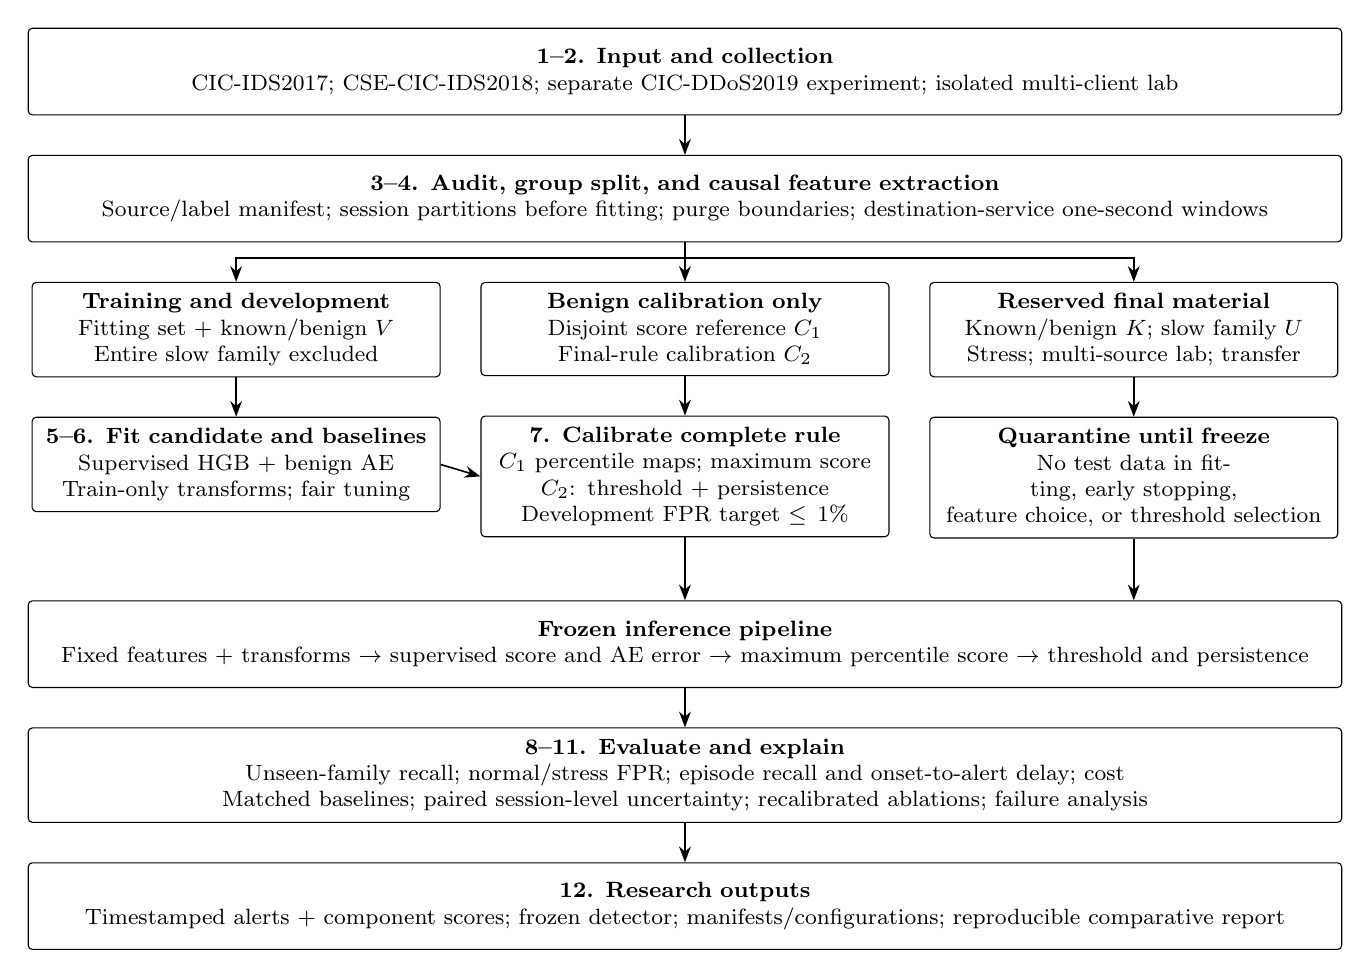
\begin{tikzpicture}[
  node distance=5mm and 7mm,
  box/.style={draw,rounded corners=1.5pt,align=center,font=\footnotesize,inner sep=4pt,minimum height=11mm},
  wide/.style={box,text width=16.4cm},
  third/.style={box,text width=4.9cm},
  half/.style={box,text width=7.6cm},
  arr/.style={-{Stealth[length=2mm]},semithick},
  note/.style={font=\scriptsize,align=center}
]
\node[wide] (data) {\textbf{1--2. Input and collection}\\CIC-IDS2017; CSE-CIC-IDS2018; separate CIC-DDoS2019 experiment; isolated multi-client lab};
\node[wide,below=of data] (audit) {\textbf{3--4. Audit, group split, and causal feature extraction}\\Source/label manifest; session partitions before fitting; purge boundaries; destination-service one-second windows};
\node[third,below=of audit,xshift=-5.7cm] (train) {\textbf{Training and development}\\Fitting set + known/benign $V$\\Entire slow family excluded};
\node[third,below=of audit] (cal) {\textbf{Benign calibration only}\\Disjoint score reference $C_1$\\Final-rule calibration $C_2$};
\node[third,below=of audit,xshift=5.7cm] (test) {\textbf{Reserved final material}\\Known/benign $K$; slow family $U$\\Stress; multi-source lab; transfer};
\node[third,below=of train] (fit) {\textbf{5--6. Fit candidate and baselines}\\Supervised HGB + benign AE\\Train-only transforms; fair tuning};
\node[third,below=of cal] (rule) {\textbf{7. Calibrate complete rule}\\$C_1$ percentile maps; maximum score\\$C_2$: threshold + persistence\\Development FPR target $\leq1\%$};
\node[third,below=of test] (hold) {\textbf{Quarantine until freeze}\\No test data in fitting, early stopping,\\feature choice, or threshold selection};
\node[wide,below=8mm of rule] (frozen) {\textbf{Frozen inference pipeline}\\Fixed features + transforms $\to$ supervised score and AE error $\to$ maximum percentile score $\to$ threshold and persistence};
\node[wide,below=of frozen] (eval) {\textbf{8--11. Evaluate and explain}\\Unseen-family recall; normal/stress FPR; episode recall and onset-to-alert delay; cost\\Matched baselines; paired session-level uncertainty; recalibrated ablations; failure analysis};
\node[wide,below=of eval] (out) {\textbf{12. Research outputs}\\Timestamped alerts + component scores; frozen detector; manifests/configurations; reproducible comparative report};
\draw[arr] (data)--(audit);
\foreach \n in {train,cal,test}{\draw[arr] (audit.south) -- ++(0,-2mm) -| (\n.north);}
\draw[arr] (train)--(fit); \draw[arr] (cal)--(rule); \draw[arr] (test)--(hold);
\draw[arr] (fit.east)--(rule.west);
\draw[arr] (rule)--(frozen);
\draw[arr] (hold.south) -- ++(0,-3mm) -| ([xshift=5.7cm]frozen.north);
\draw[arr] (frozen)--(eval); \draw[arr] (eval)--(out);
\end{tikzpicture}
\caption{Proposed research methodology. The numbered stages correspond to the twelve required methodology steps. All final experiments use frozen preprocessing, models, score mappings, threshold, and persistence. The false-positive target is a development constraint, not a guarantee on final traffic.}
\label{fig:method}
\end{figure*}

\subsection{Step 10 Ablation and component analysis}
\noindent\textit{Remove supervised branch.} Contribution of known-attack learning. Known/unseen recall and stress FPR.

\noindent\textit{Remove autoencoder branch.} Contribution of benign anomaly learning. Unseen-family recall difference.

\noindent\textit{Remove rolling history.} Value of causal temporal representation. Episode recall versus observation delay.

\noindent\textit{Remove persistence.} Value of repeated evidence. Stress FPR and detection-delay tradeoff.

\noindent\textit{Remove timing/connection features.} Whether the detector depends mainly on volume. Low-rate recall compared with volume-only inputs.

\noindent\textit{Class weights off.} Effect of imbalance treatment. Per-family recall and precision.

Retrain each applicable variant on the same groups, then recalibrate its complete final rule on the same development benign sets to the same FPR target. Keep seeds and testing fixed. Recalibration is necessary because removing a branch changes the score scale. Also show an optional fixed-threshold removal only as a diagnostic, clearly distinguished from the matched-operating-point comparison.

\subsection{Step 11 Error and failure analysis}
Inspect false positives by legitimate workload, destination, protocol and session. Inspect false negatives by excluded family, measured rate, active connections, attack duration and client count. Plot benign-stress and attack score overlap; distinguish data/label errors from model errors. Check cold-start misses, alert lag, missing features, exporter timeouts and residual identifier leakage. Examine cases where legitimate congestion and malicious resource exhaustion have similar metadata; if the available features cannot separate them, report the observability limit.

Record whether a missed lab trace actually degraded service. Keep attempted attacks and successful denial-of-service episodes distinguishable. Threshold or feature changes suggested by final-test errors belong to a future iteration requiring a new untouched test set; they are not retroactively applied to improve this study.

\subsection{Step 12 Final research output}
Produce the fitted detection pipeline, frozen feature schema, preprocessing parameters, C1 score maps, final decision threshold, model configurations, seeds and an environment file. Release scripts or notebooks for extraction, manifest generation, fitting and evaluation, plus licence-compatible dataset links and hashes. The evaluation report will include matched baseline results, per-family confusion matrices, stress FPR, recall-delay curves, paired uncertainty intervals, ablation tables and labelled failure examples.

The practical output is a timestamped destination-service alert with supervised score, reconstruction score, combined score and persistence state. The scientific output is evidence for or against the hypotheses, including situations where a simple baseline is sufficient or every method fails. No accuracy, novelty or deployment claim will be made until these measurements exist.

\section{Research Methodology Architecture}
\label{sec:architecture}
Figure 1 presents the complete proposed workflow. Arrows into the fitting and calibration branches originate only from the permitted development partitions. The quarantined slow-family test and other final sessions enter the detector after the full configuration is frozen.

\section{Feasibility and Threats to Validity}
\label{sec:validity}
\subsection{Four-Month Implementation Plan}
\noindent\textit{Weeks 1 to 2.} Audit source files, labels and licences; create family/session manifest and lab topology.

\noindent\textit{Weeks 3 to 4.} Implement causal feature extractor and grouped partitions; pilot normal and stress workloads.

\noindent\textit{Weeks 5 to 7.} Train simple baselines and both branches; complete development-only configuration search.

\noindent\textit{Weeks 8 to 9.} Construct C1/C2 mappings; calibrate final rules; freeze manifest and configurations.

\noindent\textit{Weeks 10 to 12.} Run novelty, benign-stress, distributed-source and frozen-transfer experiments.

\noindent\textit{Weeks 13 to 14.} Complete statistical comparisons, component ablations and error inspection.

\noindent\textit{Weeks 15 to 16.} Package reproducibility materials, final figures and research report.

\subsection{Threats to Validity}
Public captures may contain few independent slow-attack episodes, correlated flows, schedule-derived labels or data errors. Grouped splits, provenance audits and session-level uncertainty reduce these risks but cannot create attack diversity. An older public dataset and a small lab do not represent all operational traffic. Lab workload generators may make benign stress artificially easy; use several traffic seeds and match load ranges across benign and malicious conditions where feasible.

A false-positive target selected on development benign traffic can drift on a new network. Report transfer failure directly. Destination aggregation may dilute very weak attacks or mix simultaneous families; label ambiguous windows and examine dilution separately. CPU inference speed does not demonstrate IoT-device deployability. The core implementation is CPU-oriented; federated training, large GANs and production response integration are excluded to keep the plan feasible.

\section{Conclusion}
The extended review refines the project from a broad claim about unseen-attack detection to a measurable operating question: excluded slow-family recall under a fixed false-positive budget, including legitimate stress, temporal delay and environment change. The proposed compact hybrid is a candidate to evaluate against simple baselines. The twelve-step protocol and architecture define how positive and negative findings will be measured and reproduced. Experimental results will determine whether the hypotheses hold; no superiority is assumed at the proposal stage.

% Natural bibliography flow; recheck the final columns after content edits.
\begin{thebibliography}{18}
\bibitem{ref1} R. Bocu and M. Iavich, ``Generalized detection of DDoS attack patterns using machine learning models,\textquotedblright{} \emph{Journal of Network and Computer Applications}, vol. 248, Art. no. 104441, 2026. \url{https://doi.org/10.1016/j.jnca.2026.104441}.
\bibitem{ref2} A. Rullo, E. Cambiaso and M. Guarascio, ``Detecting the invisible without knowledge: Unsupervised packet-based real-time detection of slow DoS attacks,\textquotedblright{} \emph{Applied Soft Computing}, vol. 202, Art. no. 115796, 2026. \url{https://doi.org/10.1016/j.asoc.2026.115796}.
\bibitem{ref3} M. Nakip, ``A predictive neural network architecture for early detection of low-rate cyberattacks,\textquotedblright{} \emph{Knowledge-Based Systems}, vol. 343, Art. no. 115995, 2026. \url{https://doi.org/10.1016/j.knosys.2026.115995}.
\bibitem{ref4} M. R. Minhas et al., ``F-OSFA: A Fog Level Generalizable Solution for Zero-Day DDOS Attacks Detection,\textquotedblright{} \emph{IEEE Access}, vol. 13, pp. 75153-75166, 2025. \url{https://doi.org/10.1109/ACCESS.2025.3557822}.
\bibitem{ref5} S. Ullah et al., ``Hybrid dual-head IDS: A lightweight and explainable deep learning DDOS/DOS framework for zero-day and imbalanced attack detection in IoT networks,\textquotedblright{} \emph{Results in Engineering}, vol. 31, Art. no. 111498, 2026. \url{https://doi.org/10.1016/j.rineng.2026.111498}.
\bibitem{ref6} S. Han, S. Son, W. Sakong and H. Jung, ``Adapting Convolutional Autoencoder for DDoS Attack Detection via Joint Reconstruction Learning and Refined Anomaly Scoring,\textquotedblright{} \emph{Computers, Materials \& Continua}, vol. 85, no. 2, pp. 2893-2912, 2025. \url{https://doi.org/10.32604/cmc.2025.067211}.
\bibitem{ref7} M. Nawaz et al., ``Lightweight machine learning framework for efficient DDoS attack detection in IoT networks,\textquotedblright{} \emph{Scientific Reports}, vol. 15, Art. no. 24961, 2025. \url{https://doi.org/10.1038/s41598-025-10092-0}.
\bibitem{ref8} R. Anandhi and G. U. Srikanth, ``Federated sparse-learning framework for detecting low-rate stealth attacks in resource-constrained IoT devices,\textquotedblright{} \emph{Scientific Reports}, vol. 16, Art. no. 21298, 2026. \url{https://doi.org/10.1038/s41598-026-46531-9}.
\bibitem{ref9} M. Raza, M. A. Sattar, Z. Jahangir and M. Billah, ``Liquid neural networks for adaptive DDoS detection in IoT and SDN environments,\textquotedblright{} \emph{Scientific Reports}, vol. 16, Art. no. 26053, 2026. \url{https://doi.org/10.1038/s41598-026-67535-5}.
\bibitem{ref10} O. Ebrahem, S. Dowaji and S. Alhammoud, ``A lightweight machine learning approach for DDoS detection and classification,\textquotedblright{} \emph{Scientific Reports}, vol. 16, Art. no. 16895, 2026. \url{https://doi.org/10.1038/s41598-026-48535-x}.
\bibitem{ref11} S. A. A. Kalafy, S. Pashazadeh and P. Salehpour, ``Dynamic graph neural network-based framework to increase detection accuracy in SDN under DDOS,\textquotedblright{} \emph{Scientific Reports}, vol. 16, Art. no. 2305, 2026; first online 29 December 2025. \url{https://doi.org/10.1038/s41598-025-32102-x}.
\bibitem{ref12} Canadian Institute for Cybersecurity, Intrusion detection evaluation dataset CIC-IDS2017, official dataset description and attack schedule. Accessed 14 October 2026. \url{https://www.unb.ca/cic/datasets/ids-2017.html}.
\bibitem{ref13} Canadian Institute for Cybersecurity and Communications Security Establishment, CSE-CIC-IDS2018 on AWS, official dataset description. Accessed 14 October 2026. \url{https://www.unb.ca/cic/datasets/ids-2018.html}.
\bibitem{ref14} Canadian Institute for Cybersecurity, DDoS evaluation dataset CIC-DDoS2019, official dataset description. Accessed 14 October 2026. \url{https://www.unb.ca/cic/datasets/ddos-2019.html}.
\bibitem{ref15} SCImago Journal and Country Rank, 2024 journal ranking listing, IEEE Access, SJR 0.849, Q1. Indexed listing accessed 14 October 2026. \url{https://www.scimagojr.com/journalrank.php?country=&min=3&min_type=cd&ord=desc&order=titem&year=2024}.
\bibitem{ref16} SCImago Journal and Country Rank, 2024 United Kingdom journal ranking listing, Scientific Reports, SJR 0.874, Q1. Historical ranking rechecked 17 October 2026. \url{https://www.scimagojr.com/journalrank.php?country=GB&ord=desc&order=cd&year=2024}.
\bibitem{ref17} Comillas Institute for Research in Technology, Results in Engineering journal record, SJR 2024 1.171 Q1 and SJR 2025 1.240 Q1. Accessed 14 October 2026. \url{https://www.iit.comillas.edu/publicacion/info_revista/en/675/Results_in_Engineering}.
\bibitem{ref18} Comillas Institute for Research in Technology, Computer, Materials \& Continua journal record, SJR 2024 0.431 Q2 and SJR 2025 0.513 Q2; JCR Q3 in both years. Accessed 14 October 2026. \url{https://www.iit.comillas.edu/publicacion/info_revista/en/655/Computer%2C_Materials_%26_Continua}.
\end{thebibliography}
\end{document}
